\chapter{Referencial Teórico}
\noindent
\lipsum[15]

\section{Generalidades}

\lipsum[16]

\subsection{Conceitos da xxxxxxxxxxxxxx}

\begin{citacao}
    \lipsum[17] \cite{DoutrinaMilitarTerrestre54}.
\end{citacao}

Segundo \citeonline{DoutrinaMilitarTerrestre54} xxxxxxxxxxxxxxxxxxxxxxxxx xxxxxxxxxx xxxxxxxxx.

\begin{citacao}
    \lipsum[18] \cite{DoutrinaMilitarTerrestre54}.
\end{citacao}

\lipsum[19]



\section{Principais xxxxxxxxxx em uso na FTer}
\lipsum[20-23] \cite{LivroBrancodeDefesaNacional455,EstruturaMilitardeDefesa454}.


\section{Sistema xxxxxxxx xxxxxxxx}

\lipsum[7]


\section{Aplicações xxxxxxxxxxxxxxxx}

\lipsum[24]

\begin{figure}[!h]
    \centering
    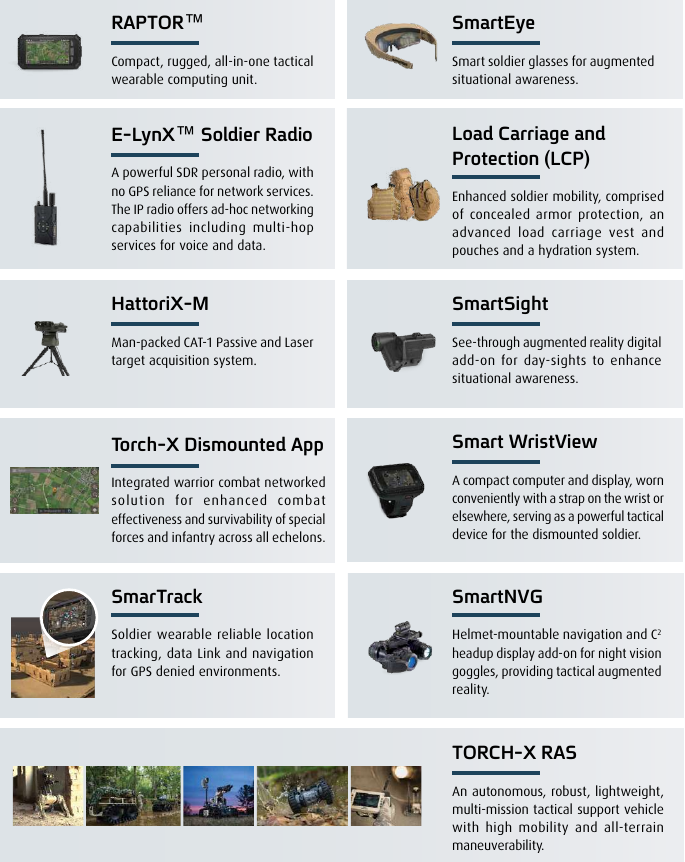
\includegraphics[width=1\linewidth]{img/torchx_dismounted}
    \caption{Datasheet do Torch X dismounted com os principais elementos integradores do sistema.}
    \legend{Fonte: \cite{TorchXDs}}
    \label{fig:torchxdismounted}
\end{figure}

\lipsum[25]

\begin{figure}[!h]
    \centering
    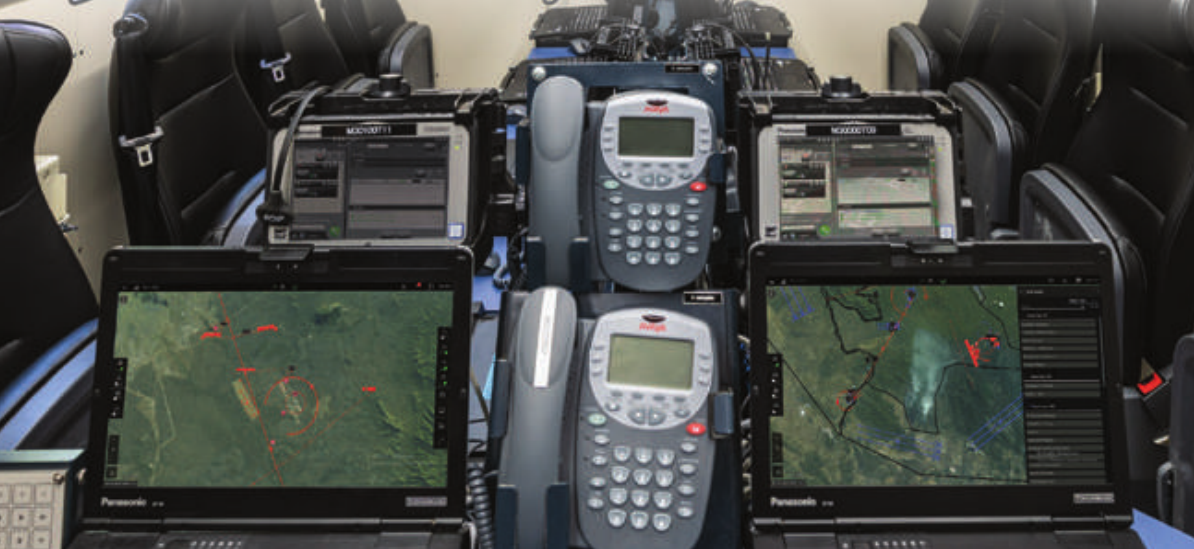
\includegraphics[width=1\linewidth]{img/torchx}
    \caption{Torch X HQ em operação}
    \legend{Fonte: \cite{TorchXHQ}}
    \label{fig:torchxhd}
\end{figure}

\lipsum[26]

\begin{figure}[!h]
    \centering
    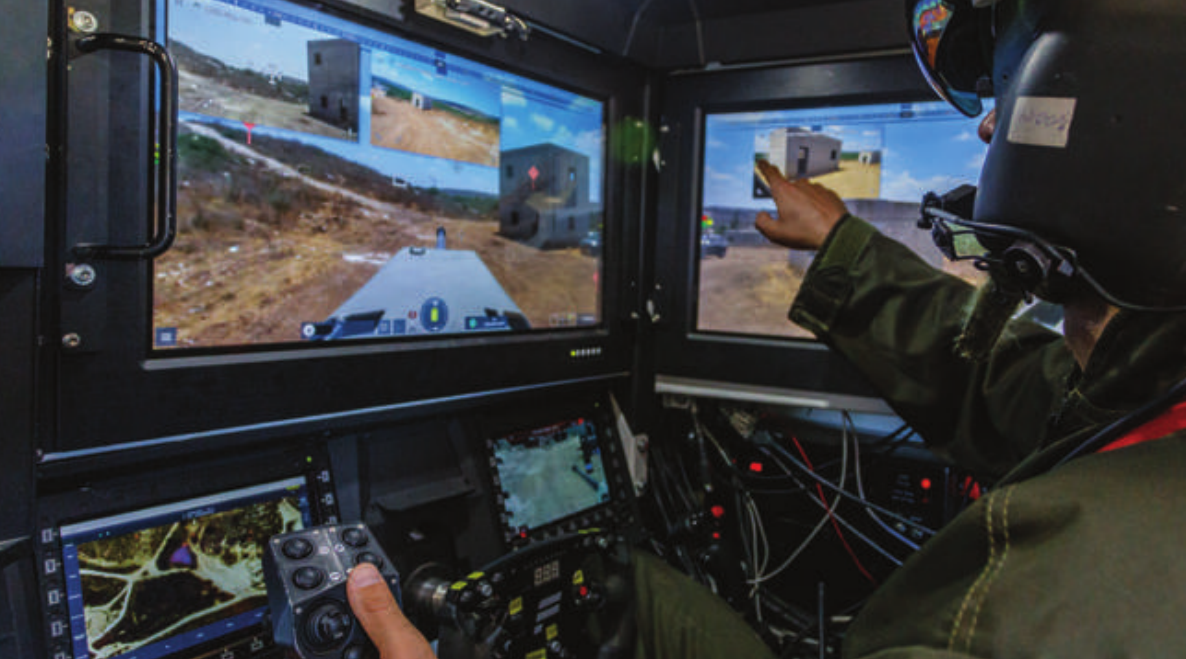
\includegraphics[width=1\linewidth]{img/torchx_mounted}
    \caption{Torch X Mounted}
    \legend{Fonte: \cite{TorchX}}
    \label{fig:torchxmounted}
\end{figure}

\lipsum[27]

\section{xxxxxxxx xxxxxxxxxxxxx}

\subsection{Conceitos de xxxxxxxx}

\lipsum[25-30]

\begin{equation}
    \label{math:acuracia}
    AccC_1 = \frac{VP + VN}{n}
\end{equation}


\begin{equation}
    \label{math:abrangencia}
    RevC_1 = \frac{VP}{VP+FN}
\end{equation}



\begin{equation}
    \label{math:precisao}
    PrecC_1 = \frac{VP}{VP+FP}
\end{equation}


\begin{equation}
    \label{math:f1}
    F_1 = \frac{2*Prec*Rev}{Prec + Rev}
\end{equation}

\lipsum[31]

\begin{table}[!ht]
    \centering
    \caption{Matriz de xxxxxxxxx}
    \label{tab:matriz_de_xxxxxx}
    \vspace{0.5cm}
    \begin{tabular}{r|cccc||c}
        & P ($ C_1 $)   & P ($ C_2 $)   & Total Real \\
        \hline
        \hline
        R ($ C_1 $)             & (VP) 120 & (FN) 40  & 160      \\
        R ($ C_2 $)             & (FP) 33  & (VN) 127 & 160      \\
        \hline
        \hline
        Total xxxxxx & 153 & 167 & 320      \\
        \hline
    \end{tabular}
\end{table}
